\chapter{Web Application}
To provide an accessible and user-friendly means of leveraging our vehicle price prediction model, we developed a web application designed for end-users. The primary functionality of this web application is to facilitate inference through an intuitive user interface and well-documented API endpoints.

\section{Architecture}
To ensure a scalable and maintainable solution, we designed our web application using a RESTful architecture. This approach allows for a clear separation of concerns between the frontend and backend, ensuring that the user interface (UI) remains independent of the underlying logic and data processing.

Representational State Transfer (REST) is an architectural style that uses standard HTTP methods to interact with resources, which are identified by URLs. Our backend exposes several RESTful endpoints that allow for interaction with the model and other functionalities of the application. These endpoints handle various operations, including data retrieval, model inference, payment and user authentication.

\section{Backend}
Considering our target clients, which include both our users and other businesses, we aimed to create a robust solution that could seamlessly integrate with any user interface. To achieve this, we developed a web application programming interface (API) that exposes our inference model, allowing clients to utilize it in various scenarios according to their needs.

\subsection{Tech Stack}
To ensure our backend could efficiently serve not only our client application but also external frontends, we chose \textit{FastAPI} \cite{fastapi} as our framework. FastAPI offers a multitude of advantages, including the automatic generation of interactive API documentation through Swagger, which provides comprehensive and easily navigable documentation for each endpoint when properly configured.

Our decision to remain within the Python ecosystem was driven by the need for seamless integration with machine learning packages. After considering Django, Flask, and FastAPI, we opted for FastAPI due to several compelling reasons:

\begin{itemize}
    \item \textbf{Performance}: The web, fundamentally based on HTTP requests, poses an I/O-bound heavy task for any web server. One of the standout features of FastAPI is its support for asynchronous programming, making it unique among Python web frameworks. This capability allows FastAPI to handle numerous simultaneous requests efficiently, reducing latency and improving overall performance. This, combined with its lightweight nature and the flexibility to choose all the other tools, makes it the most performant Python web framework available
    \item \textbf{Ease of use}: At its core, FastAPI addresses one of Python's long-standing challenges: the lack of static typing. Although type hints were introduced in Python 3.5, they do not provide the same level of static type enforcement as statically typed languages like C or Go. This often complicates the development process, making it more error-prone and less efficient. FastAPI, however, leverages type hints extensively, enhancing the developer experience significantly. By using type hints, FastAPI enables better code validation and error checking, akin to the benefits found in statically typed languages. Additionally, FastAPI offers an intuitive and modern approach to creating APIs through Python decorators. This makes defining endpoints straightforward and expressive, allowing us to build APIs with minimal boilerplate code.
    \item \textbf{Granularity and Flexibility}: Unlike Django, which is a comprehensive framework that includes built-in database adapters, an ORM, and migration tools, FastAPI provides developers with the freedom to choose their own tools and packages. This modularity allows for greater customization and flexibility, enabling developers to select the best components for their specific needs rather than being constrained by the framework’s built-in features.
    \item \textbf{Validation and Serialization}: Powered by \textit{Pydantic} \cite{pydantic}, FastAPI ensures robust data validation and serialization, reducing the likelihood of runtime errors and improving data integrity.
    \item \textbf{Interactive API Documentation}: One of the standout features of FastAPI is its automatic generation of interactive API documentation. Utilizing \textit{OpenAPI} \cite{openapi} and JSON Schema standards, FastAPI creates a detailed and interactive documentation interface with \textit{Swagger UI} \cite{swagger}.
\end{itemize}

\subsection{Architecture}
For our architecture, we adopted a modular approach. In line with the core principles of \textit{Clean Code} \cite{clean_code} by Robert C. Martin, which emphasize high readability, maintainability, and modularity, we chose to divide our logic into distinct modules. This approach not only enhances the clarity and organization of our codebase but also facilitates easier testing, debugging, and future enhancements. By breaking down the functionality into smaller, self-contained units, we ensure that each module adheres to the \textit{Single Responsibility Principle}, making the overall system more robust and adaptable to change.

\begin{itemize}
    \item \textbf{Schemas Module}: This module is responsible for configuring and defining all our API schemas, including request and response schemas for both successful operations and errors. It ensures that data structures are consistent and well-documented throughout the API.
    \item \textbf{APIs Module}: In this module, we define all our API endpoints and their associated documentation. It serves as the central hub for routing and handling API requests, ensuring that each endpoint is clearly documented and easily accessible.
    \item \textbf{Services Module}: This module contains the business logic and is invoked by our API endpoints. It acts as a bridge between user inputs and the repository module, processing the inputs and implementing the core functionalities of our application.
    \item \textbf{Repositories Module}: Called exclusively by our services, this module is responsible for all database interactions. It encapsulates the logic for data retrieval, storage, and manipulation, ensuring a clean separation of concerns.
    \item \textbf{S3 Module}: This data module is dedicated to configuring and managing our AWS S3 storage. It handles the download of processors and models at startup, providing essential resources for our application.
    \item \textbf{Auth Module}: This module handles the business logic for authentication. It manages user credentials, session management, and authorization processes, ensuring secure access to the application's features.
    \item \textbf{Models Module}: Utilizing an ORM (Object-Relational Mapping), this module is where our data models are defined and managed. It maps the database schema to Python objects, simplifying database operations.
    \item \textbf{Testing Module}: This module is dedicated to maintaining comprehensive tests, including both unit tests and integration tests. It helps us adhere to the single responsibility principle by isolating test configurations and ensuring that all aspects of the application are thoroughly tested.

\end{itemize}

The architecture is also presented in \hyperref[fig:backend-design]{Figure 5.1}.
\begin{figure}[ht]
    \centering
    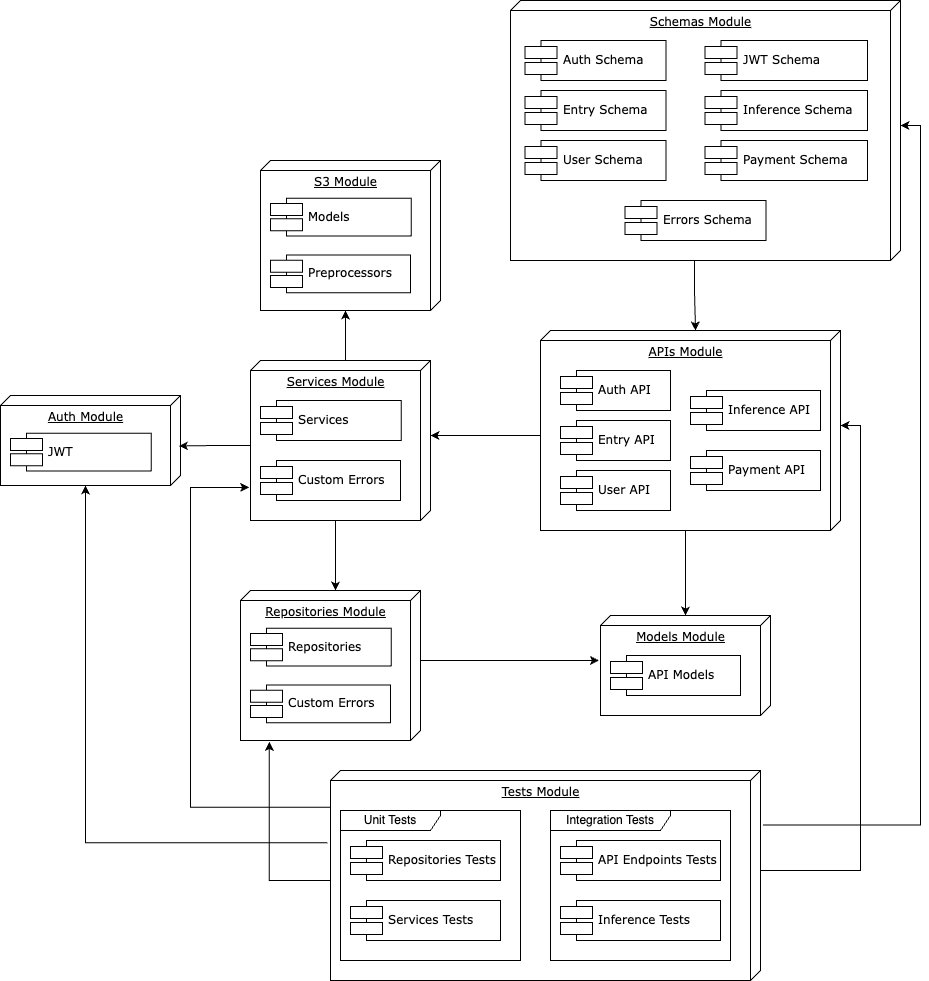
\includegraphics[width=0.8\linewidth]{images/webapp/backend/backend-modules.png}
    \caption{Backend Design}
    \label{fig:backend-design}
\end{figure}

For better scalability, we leveraged \textit{"Clean Code"} lessons further by creating abstractization layers for common tasks such as CRUD operations. This helps our app avoid code duplication and offers a better starting point for easy scalability in future updates.

In \hyperref[fig:backend-repositories]{Figure 5.2}, our abstractization is presented, along with our current services and repositories.

\begin{figure}[ht]
        \begin{subfigure}[b]{0.57\linewidth}
            \centering
            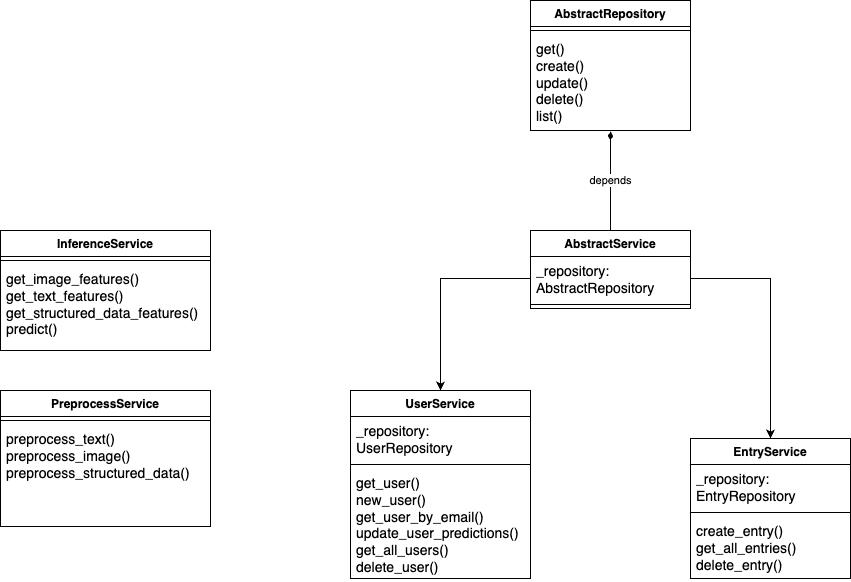
\includegraphics[width=\linewidth]{images/webapp/backend/services.png}
            \label{fig:backend-services}
        \end{subfigure}
        \hfill
        \begin{subfigure}[b]{0.43\linewidth}
            \centering
            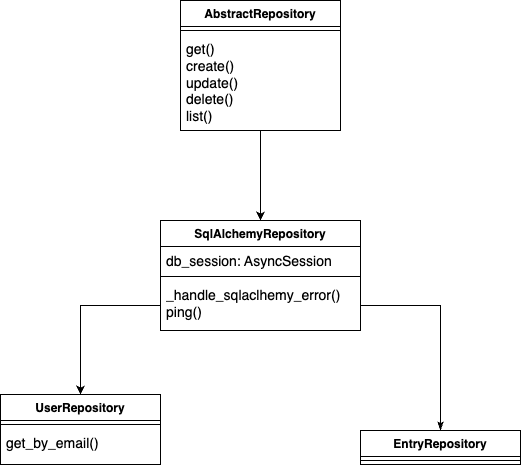
\includegraphics[width=\linewidth]{images/webapp/backend/repositories.png}
            \label{fig:backend-repositories}
        \end{subfigure}
        \caption{Services and Repositories}
        \label{fig:backend-design}
    \end{figure}

\subsection{Endpoints}
The \textit{RoCar API} exposes multiple endpoints, each with a distinct role, enabling seamless interaction with various functionalities of our application. All endpoints are prefixed with /api/v1 to ensure backward compatibility in future updates, preventing breaking changes. In this section, we will delve deeper into the specifics of each endpoint.

\subsubsection{Auth API}
The Auth API module manages the authentication processes, ensuring secure access to the application.
\begin{itemize}
\item \textbf{POST /login} - Validates user credentials and issues a JWT token upon successful authentication. This token is used for subsequent authenticated requests.
\item \textbf{POST /register} - Creates a new user account and returns a JWT token, enabling the user to access the application immediately after registration.
\end{itemize}

\subsubsection{User API}
The User API module provides endpoints for accessing user information.
\begin{itemize}
\item \textbf{GET /user/me} - Retrieves the current user's details, such as email, username, and the number of predictions remaining. This endpoint helps users verify their account information.
\end{itemize}

\subsubsection{Entry API}
The Entry API module allows users to manage their prediction entries.
\begin{itemize}
\item \textbf{GET /entry/all} - Fetches all previous predictions made by the user, allowing them to review their history and track their usage.
\item \textbf{DELETE /entry/{id}} - Deletes a specific prediction entry identified by its ID, giving users control over their data.
\item \textbf{POST /upload} - Uploads an image to the S3 bucket and returns its URL. This endpoint supports the integration of images into predictions, enhancing the model's accuracy.
\end{itemize}

\subsubsection{Payment API}
The Payment API module handles payment processes and interactions with the Stripe API \cite{stripe_api}. The entire payment integration flow can be visualised in \hyperref[fig:backend-stripe]{Figure 5.3}.

\begin{itemize}
\item \textbf{POST /create-checkout-session} - Initiates a checkout session with Stripe, providing a redirection link for the user to complete the payment. This ensures a secure and streamlined payment process.
\item \textbf{POST /webhook} - Listens for events from the Stripe API, such as successful or failed payments, and updates our system accordingly. This endpoint ensures that payment statuses are accurately reflected in our application.
\end{itemize}

\begin{figure}[ht]
    \centering
    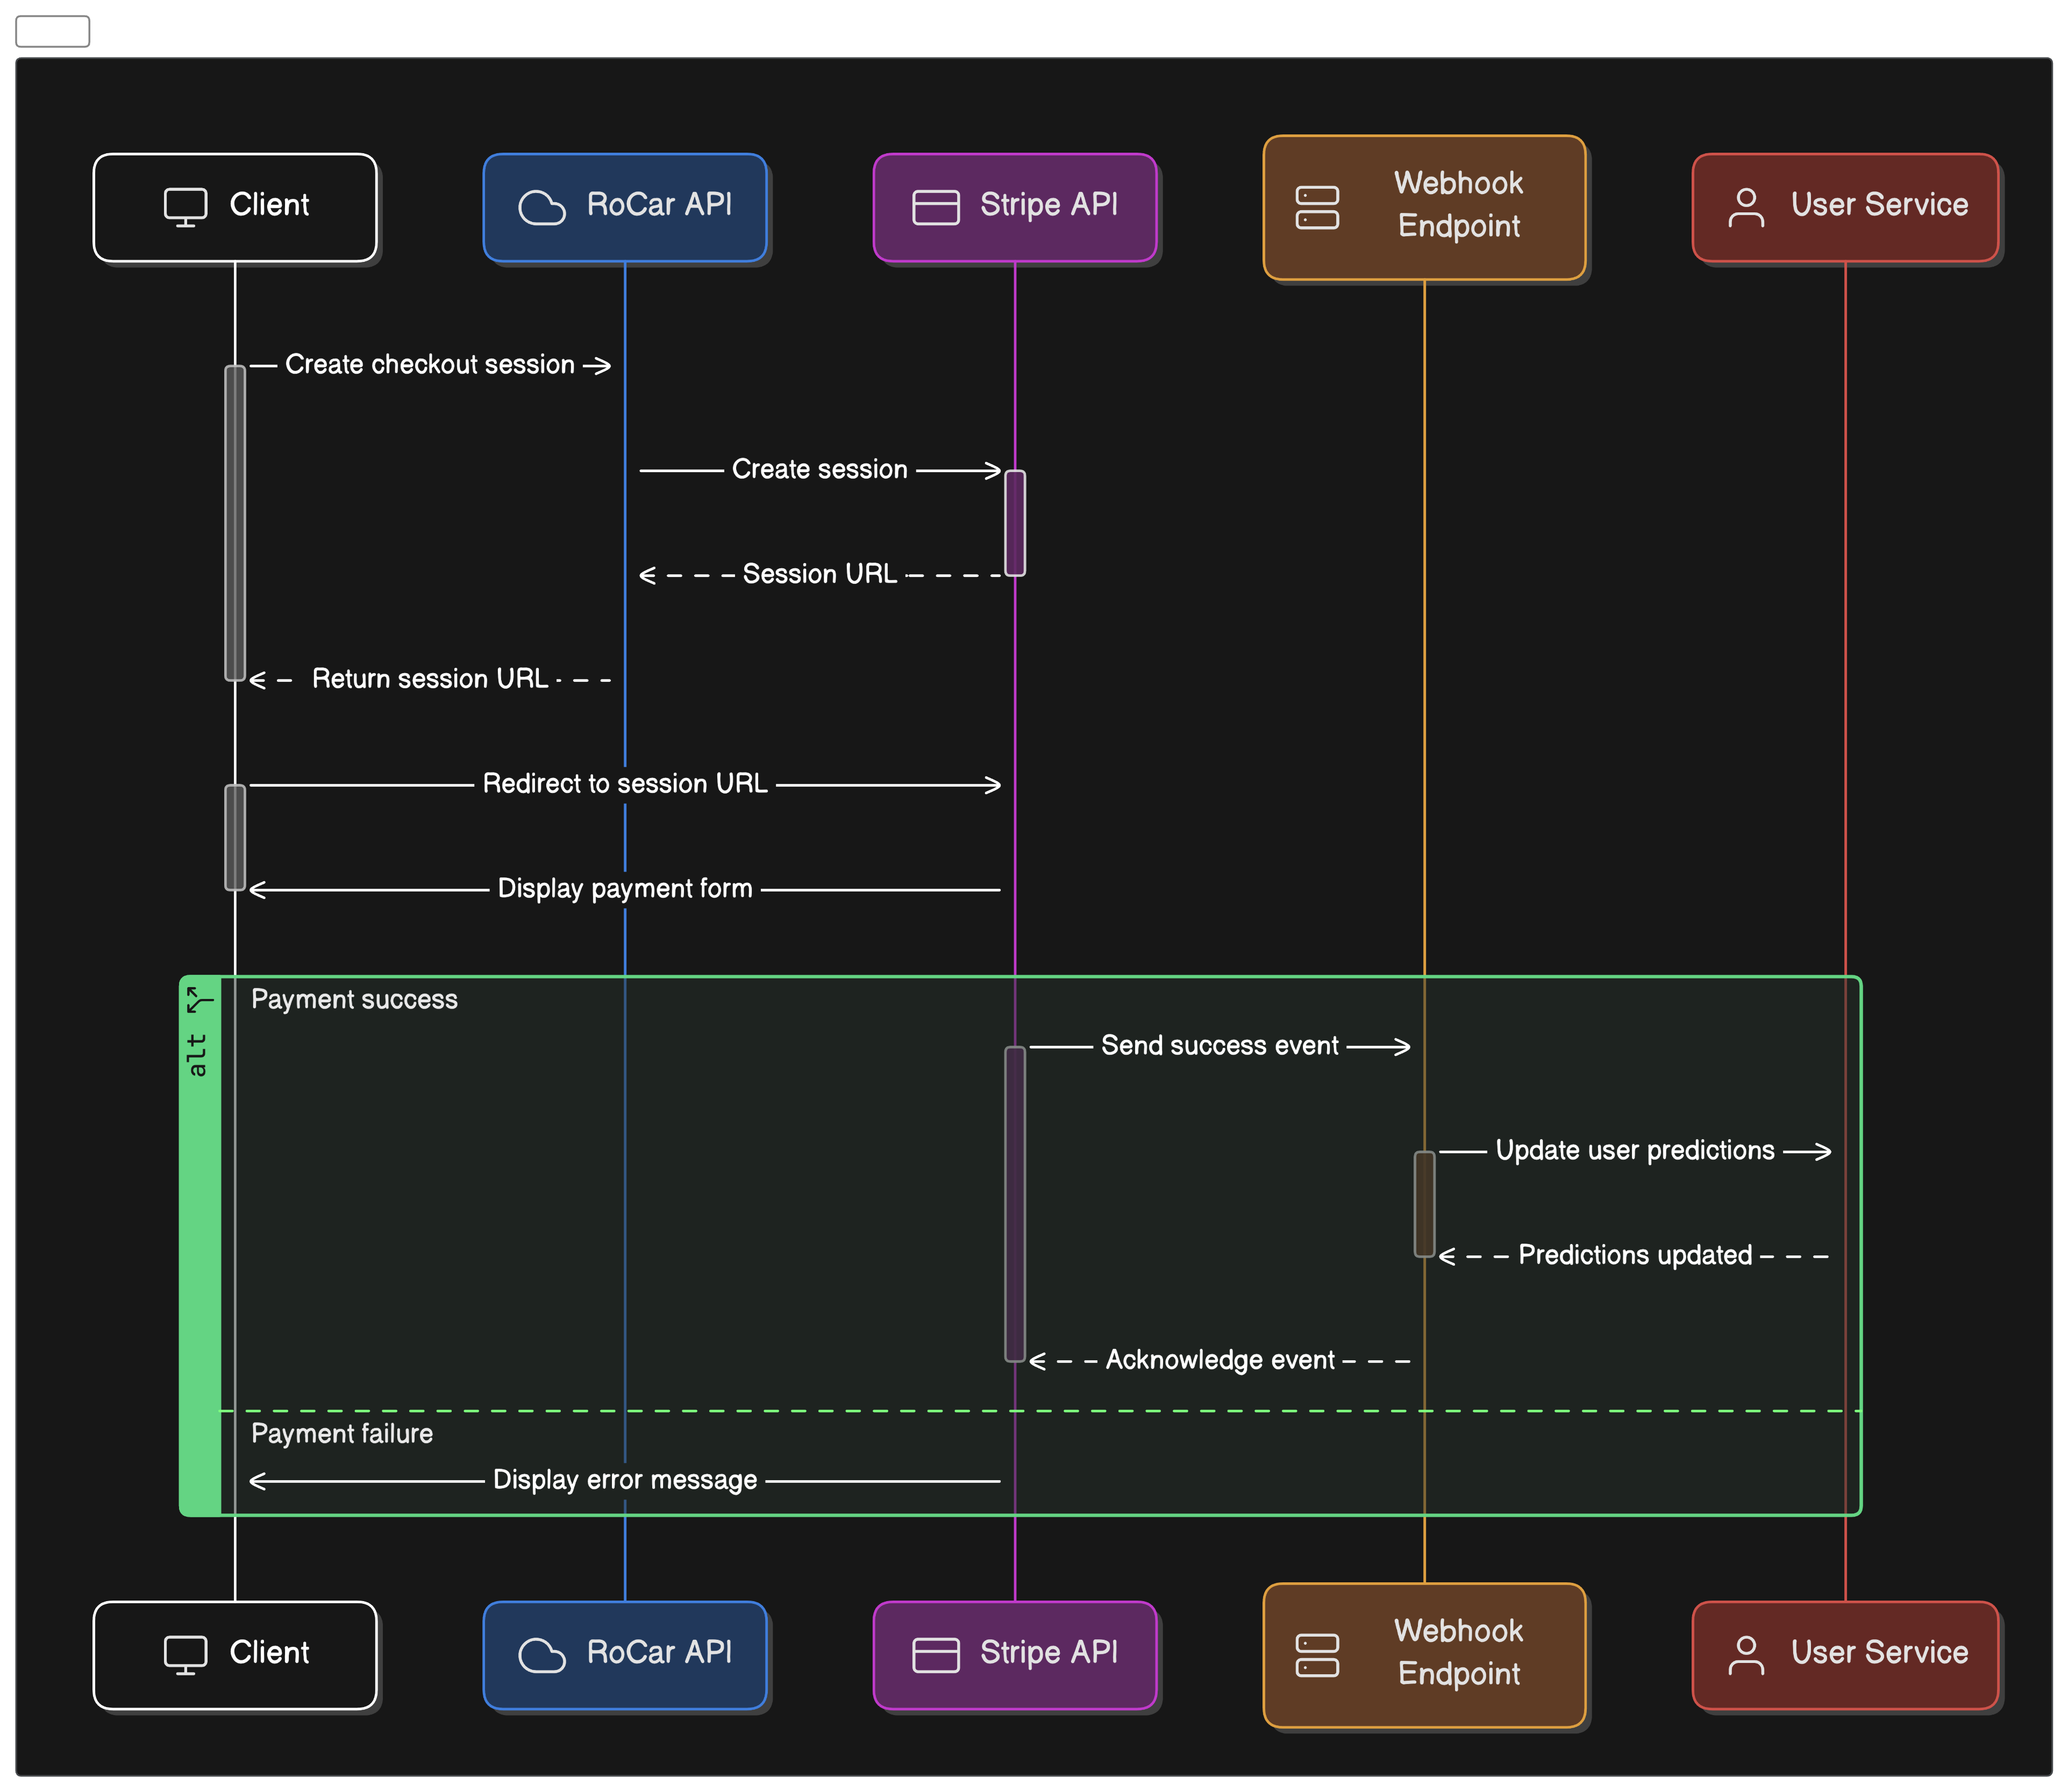
\includegraphics[width=0.7\linewidth]{images/webapp/backend/stripe.png}
    \caption{Stripe Flow}
    \label{fig:backend-stripe}
\end{figure}

\subsubsection{Inference API}
\begin{itemize}
    \item \textbf{POST /inference} - Gets the prediction of a car based on the inputs.
\end{itemize}

As our core functionality, we will showcase how it works in the next snippet.
\begin{lstlisting}
curl -X 'POST' \
  'http://127.0.0.1:8000/api/v1/inference' \
  -H 'accept: application/json' \
  -H 'Authorization: Bearer eyJhbGciOiJIUzI1...' \
  -H 'Content-Type: application/json' \
  -d '{
  "manufacturer": "audi",
  "model": "a3",
  "fuel": "gasoline",
  "chassis": "sedan",
  "sold_by": "company",
  "gearbox": "automatic",
  "km": 100000,
  "power": 160,
  "engine": 1984,
  "year": 2018,
  "description": "test description",
  "image_url": "https://thesis-s3.s3.eu-central-1.amazonaws.com/images/image.webp",
  "audio_and_technology": ["apple carplay", "infotainment system"],
  "comfort_and_optional_equipment": ["heated steering wheel"],
  "electronics_and_assistance_systems": ["rear sensors"],
  "performance": ["alloy wheels 17"],
  "safety": ["abs", "esp"]
}'

{
  "prediction": 15839
}
\end{lstlisting}

\subsection{RDBMS}
To efficiently manage and organize the data throughout our application, we selected a robust relational database management system (RDBMS) stack. The chosen stack comprises \textit{PostgreSQL} \cite{postgresql} as the database, \textit{SQLAlchemy} \cite{sqlalchemy} as the Object-Relational Mapping (ORM) library, \textit{Alembic} \cite{alembic} for database migrations, and \textit{Amazon S3} \cite{amazon_s3} for image storage.

\begin{itemize}
    \item \textbf{PostgreSQL}: We opted for PostgreSQL as our database due to its open-source nature, strong community support, and advanced features. PostgreSQL is known for its reliability, scalability, and compliance with SQL standards.
    \item \textbf{SQLAlchemy}: To interact with the PostgreSQL database, we used SQLAlchemy, a powerful ORM library for the Python ecosystem. SQLAlchemy simplifies database operations by allowing us to interact with the database using Python objects instead of writing raw SQL queries. This enhances code readability and maintainability, enabling more efficient development processes.
    \item \textbf{Alembic}: Database schema changes are a common requirement during the development lifecycle. Alembic, a database migration tool, integrates seamlessly with SQLAlchemy to manage database schema changes. It allows for the automatic generation of migration scripts, ensuring that database schema updates are consistent and easily reproducible across different environments.
    \item \textbf{Amazon S3}: For storing images associated with car advertisements, we utilized Amazon S3. S3 provides a highly scalable and durable storage solution, capable of handling large volumes of image data. Its integration with our RDBMS stack ensures that images are securely stored and easily accessible for display within our application.
\end{itemize}

Implementing the RDBMS stack involved several key steps to ensure seamless integration and optimal performance:

\begin{itemize}
    \item \textbf{Database Schema Design}: We designed a normalized database schema in PostgreSQL, focusing on minimizing redundancy and ensuring data integrity. Our current database consists of only two tables, one for the user and one for entry, connected by a one-to-many relationship. Although it is a really simple schema at the time of writing, it can be easily scaled by adapting our models module and running the migrations.
    \item \textbf{ORM Configuration}: SQLAlchemy was configured to map the database tables to Python classes present in our Models module, enabling object-oriented interaction with the database.
    \item \textbf{Migration Management}: Alembic was used to manage database migrations, ensuring that schema changes were consistently applied across all development, testing, and production environments. Automated migration scripts were generated to handle schema updates, reducing the risk of manual errors.
    \item \textbf{Image Storage Integration}: Amazon S3 was integrated into the stack for image storage. Metadata for images, such as URLs, were stored in the PostgreSQL database, while the actual image files were securely stored in S3. This separation allows for efficient data management and retrieval.
\end{itemize}

\subsection{Testing}
Testing is a crucial aspect of the development lifecycle, especially for a production-ready application. Our focus was not only on creating tests that pass but also on simulating a real production environment. This approach ensures that any changes we make do not break existing functionality, thereby maintaining the stability and reliability of our application.

We utilized the power of \textit{pytest} \cite{pytest} and \textit{pytest-asyncio} \cite{pytest_asyncio} for their easy configuration, effective mocking capabilities, and fast testing speeds. Our testing strategy includes both unit tests and integration tests to comprehensively validate our application.

\subsubsection{Unit tests}
In our unit tests, we concentrated on testing the core functionality of our services and repositories. Mocking was our primary method for handling external dependencies, allowing us to isolate and test individual components effectively.

\begin{itemize}
    \item \textbf{Focus}: The primary focus was on ensuring that each module behaves as expected in isolation.
    \item \textbf{Coverage}: Our unit tests achieve a coverage of 99\%, with all 30 tests passing consistently.
    \item \textbf{Tools}: We utilized mocking extensively to simulate external services and dependencies, ensuring that tests are self-contained and reliable.
\end{itemize}

\subsubsection{Integration tests}
To simulate a real production environment during testing, we set up a dedicated database before running integration tests. This setup was achieved using a custom Docker Compose configuration file and a custom Docker image for our application.

For an easier testing process, we create a custom script that does all the steps for us, from starting the test database, to cleaning pycache and saving the coverage for us.

The script is made with the task runner \textit{poethepoet} \cite{poethepoet}, that has it's config inside the pyproject.toml file from our virtual environment managed with \textit{poetry} \cite{poetry}.

We used this tool for various repetead cli commands, for an easier development experience:

\begin{lstlisting}[language={}]
CONFIGURED TASKS
  clean                    Clean up the project
  clean_pycache            Clean up the project of all __pycache__ folders
  unit_test                Clean artifacts and run unittests
    --cov-report           Generate coverage html or xml report
  build_image              Build docker image
    --tag                  Tag of the docker image [default: latest]
  start_app                Start the app
  stop_app                 Stop the app
  integration_test         Run API tests in a new environment
    --cov-report           Generate coverage html or xml report
  create_migration         Create migration
  upgrade_schema           Upgrade database schema
  downgrade_schema         Downgrade database schema
\end{lstlisting}

\begin{itemize}
    \item \textbf{Environment Simulation}: By spinning up a database and other necessary services, we created an environment that closely mimics production, allowing us to test the interactions between various components in a real world scenario.
    \item \textbf{Isolation}: Each test is designed to run independently, with no dependencies on other tests. This isolation ensures that tests do not pass or fail due to side effects from other tests.
    \item \textbf{Coverage}: Our integration tests achieve a coverage of 99\%, with all 32 tests passing consistently.
    \item \textbf{Tools}: We used Docker and Docker Compose to manage the setup and teardown of the testing environment, ensuring consistency and repeatability.
\end{itemize}

By employing a comprehensive testing strategy that includes both unit and integration tests, we ensured that our application is robust, reliable, and ready for production. This approach helps us maintain high code quality and quickly identify and resolve issues, providing confidence in the stability of our system.

\subsection{Deployment}
For our API we employed an automatic deployment, managed with \textit{Github Actions} \cite{github_actions}. We created rules, and jobs that check our code quality, runs tests, and sends a signal to \textit{Render} \cite{render} (our deployment platform) to pull the changes and run the deployment.

On Render, our app is deployed by it taking our custom docker image from our github repository. There we have set up a multi staged docker image, that has 3 stages.

\begin{itemize}
    \item \textbf{Base}: In the base stage we make sure poetry is installed in our container.
    \item \textbf{Development stage}: This stage is for developers, any contributor can pull the repository and run this stage step for an easy development without any additional setup.
    \item \textbf{Prepare Production Stage}: For our production environment, we aim to be as close to the metal as possible to enhance security. Therefore, this step removes Poetry and installs the dependencies using pip. We use the python:3.12-slim image to minimize security risks associated with larger base images.
    \item \textbf{Production Stage}: This is the final stage, where we utilize the dependencies installed in the previous step and start our server. A custom bash script is executed to first run migrations and then start the server.
\end{itemize}

An essential aspect of our deployment, and indeed across all our environments, is the loading process for our models and preprocessors. Before starting the server, we verify if the latest model and preprocessors are already present on the server. If they are, we proceed with the server startup. If not, we initiate the download process from our manually maintained S3 bucket. This workflow is consistently applied in local development, \textit{Docker} \cite{docker} development, testing environments, and production environments.


Our Github Actions setup is visually illustrated in \hyperref[fig:backend-cicd]{Figure 5.4}.
\begin{figure}[ht]
    \centering
    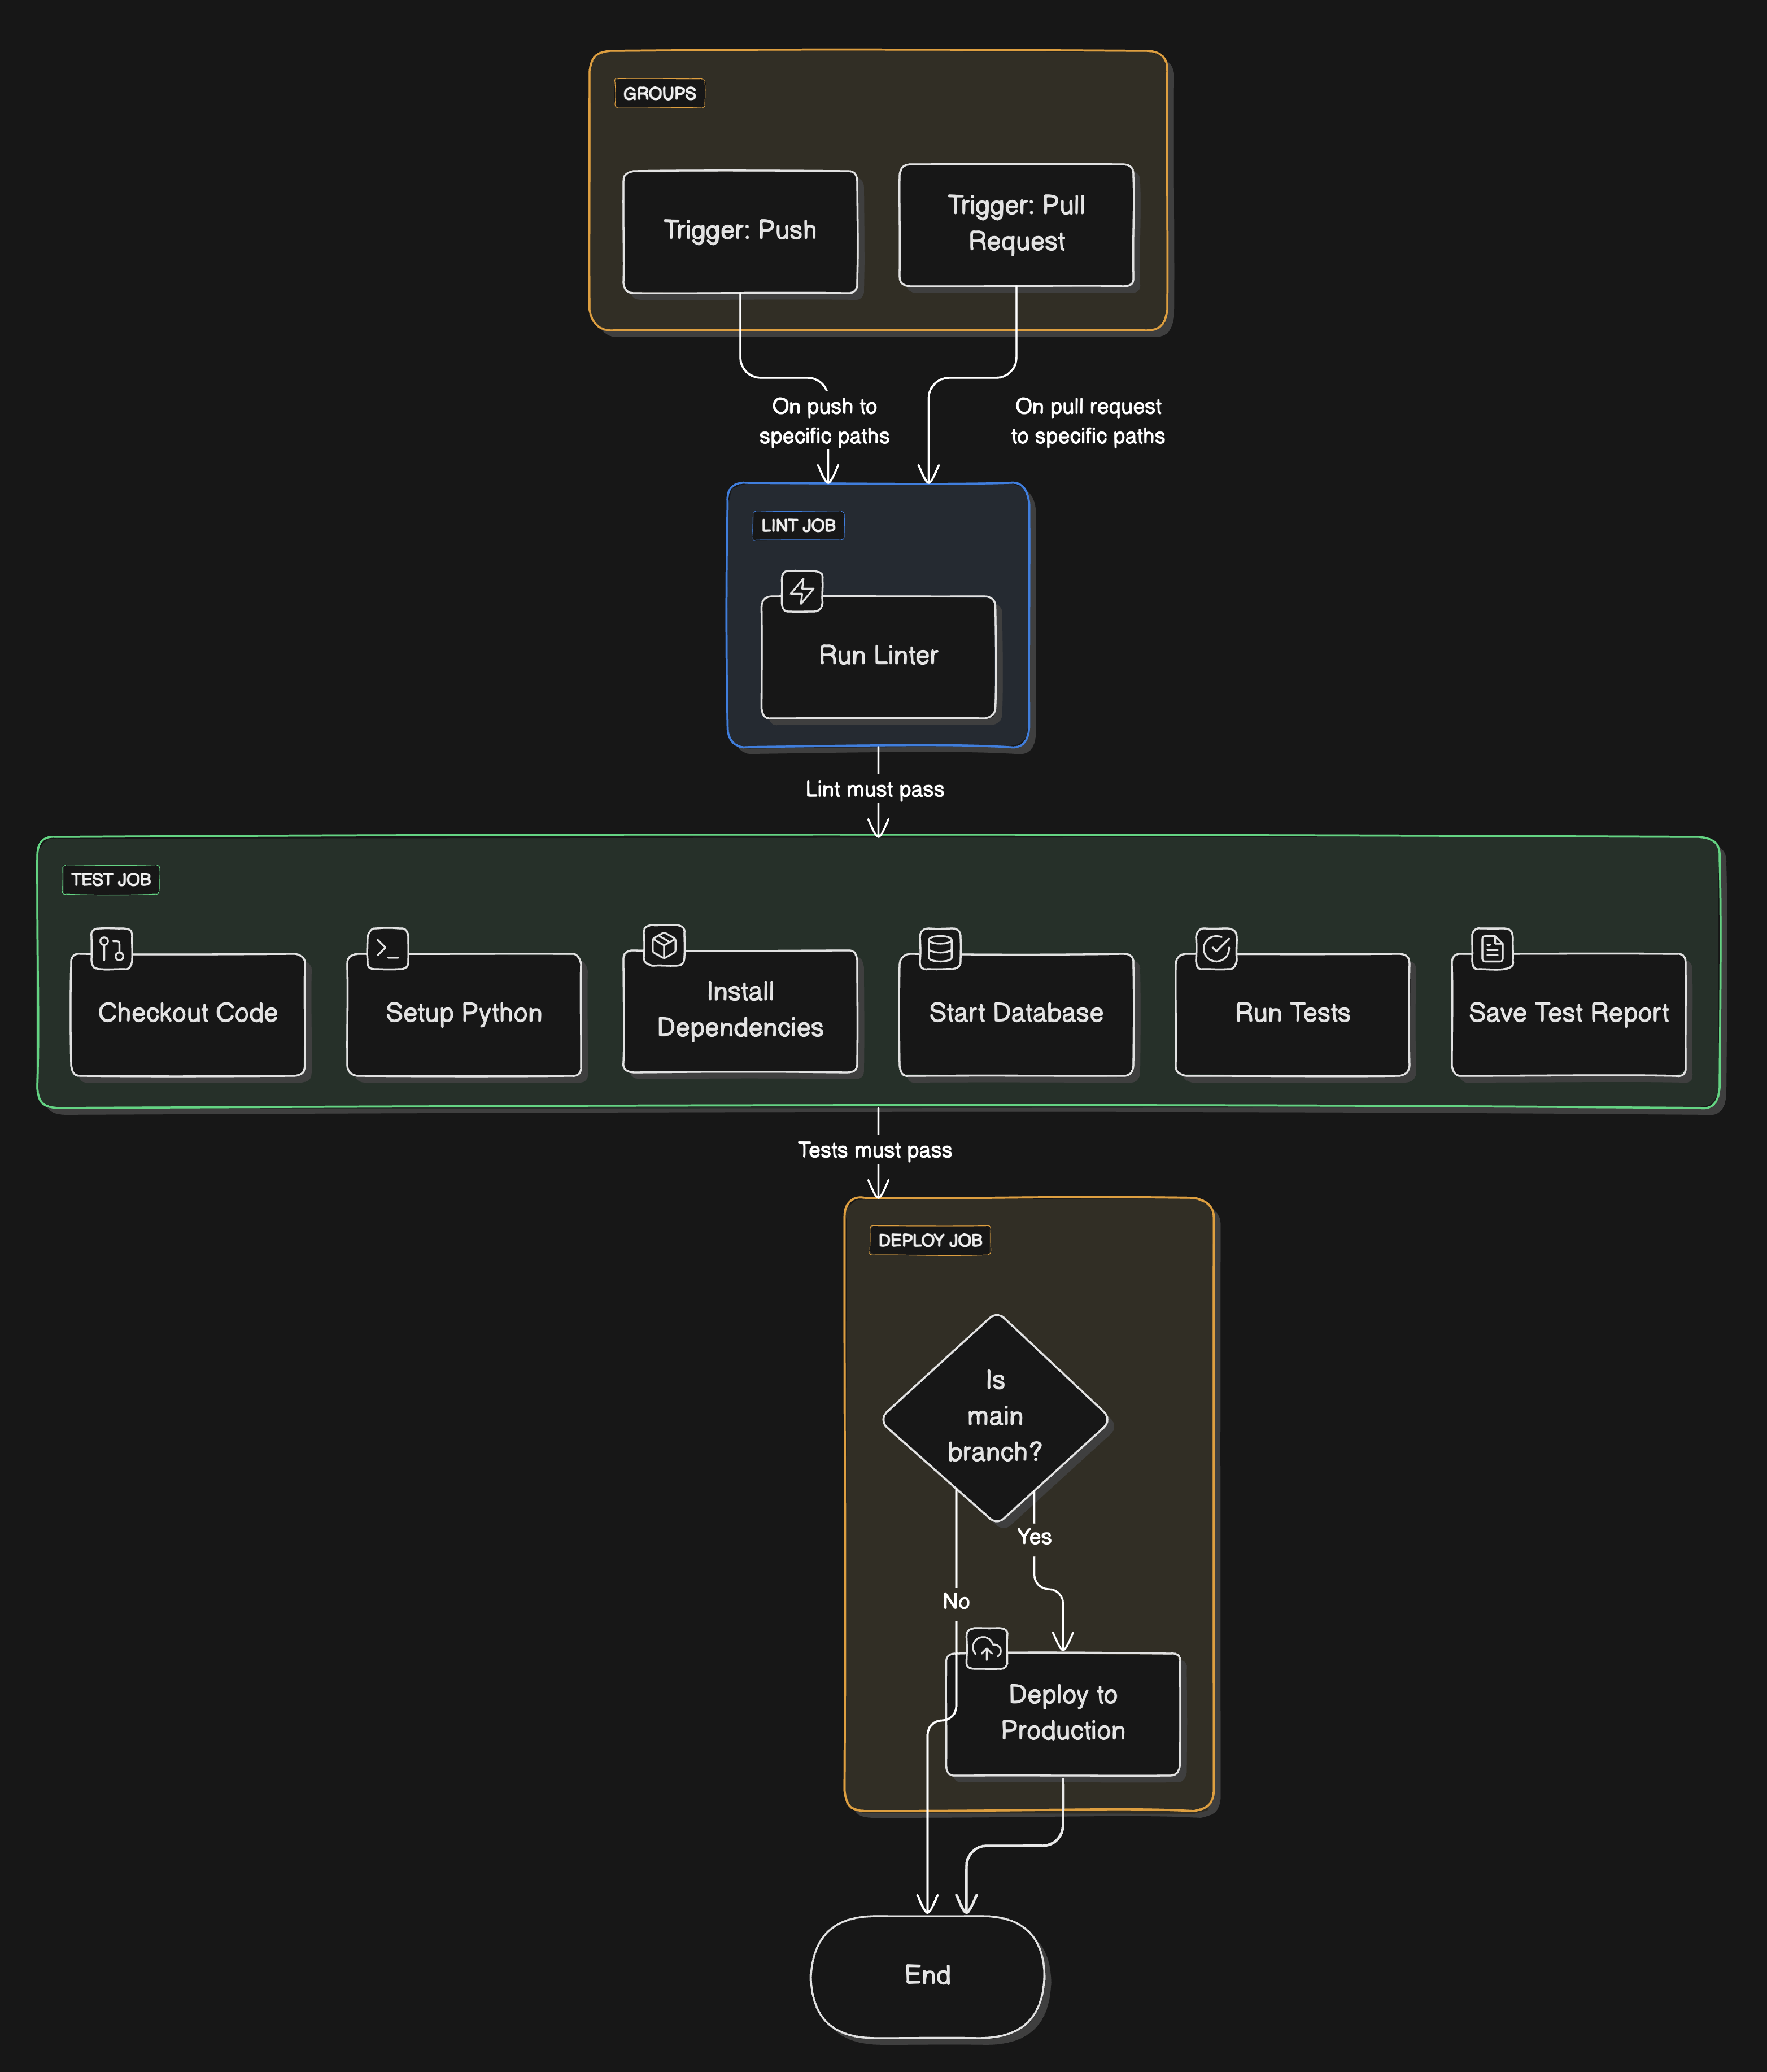
\includegraphics[width=\linewidth]{images/webapp/backend/cicd.png}
    \caption{Github Actions Pipeline}
    \label{fig:backend-cicd}
\end{figure}


\subsection{Environments}
All secrets within our app are securely stored in ignored .env files in the local environment, in GitHub secrets within our remote repository, and in Render and Vercel secrets for our deployment services. This ensures that sensitive information, such as our secret key for generating JWTs, remains protected. We maintain separate .env files for each stage: testing, development, and production, that are injected accordingly using our custom cli commands.

\section{Frontend}
In addition to the logic and functionality provided by our API, we recognized the need to make our model accessible to non-technical users. To achieve this, we developed a minimal, responsive user interface that ensures ease of use across all devices. This intuitive interface empowers users of all technical backgrounds to seamlessly interact with our model, providing a streamlined and user-friendly experience.

\subsection{Tech Stack}
Our tech stack features \textit{Next.js} \cite{nextjs}, a comprehensive framework built on React. Next.js provides significant value out of the box, including features such as caching, server-side rendering (SSR), and support for React Server Components. These capabilities ensure fast, dynamic, and SEO-friendly web applications.

In terms of our UI library, we opted for \textit{Shadcn} \cite{shadcn}. Shadcn is a headless component library that allows for complete control over styles. It leverages \textit{Tailwind CSS} \cite{tailwind_css}, providing a highly customizable and efficient styling solution.

\subsection{Pages}
The user interface comprehends six pages:

\begin{itemize}
    \item \textbf{Login page}: The page where users log in with their existing accounts.
    \item \textbf{Register page}: The page where users create accounts and then are redirected to their dashboard.
    \item \textbf{Landing page}: A public route landing page where we market our application.
    \item \textbf{Pricing page}: A public route pricing page, where users can see our pricing models. When not authenticated, they can still see the page, but if they want to buy one of our packages, they are redirected to the login page.
    \item \textbf{Dashboard page}: A private route page where authenticated users can see their old predictions made within our app.
    \item \textbf{Prediction page}: A private route page where the users are prompted with a rather big form where they insert the necessary information for the prediction.
\end{itemize}

\subsection{Deployment}
The deployment platform for our user interface is \textit{Vercel} \cite{vercel}. We connected the Vercel project to our repository, and each time a change is seen in the main branch in our frontend directory, the automatic deployment process starts. Vercel offers zero downtime deployment out of the box, an important requirement for a production ready application.
